\clearpage
% Keep the section opening with its first comparison.
\section{Complete Visual Comparisons and Hierarchical Ordering}\label{sec:full_visual_comparisons}
The main paper focuses on RG-MTM-P/R and their source fields. This section retains the complete shared-input comparisons with TMTM and ST-MTM, additional source sections, and the clustering-hierarchy example. All panels use the same frozen scientific arrays as the main results. The baselines are local reimplementations, rather than images copied from the reference publications.

\subsection{Two-dimensional inputs and controls}
\begin{figure}[H]
\centering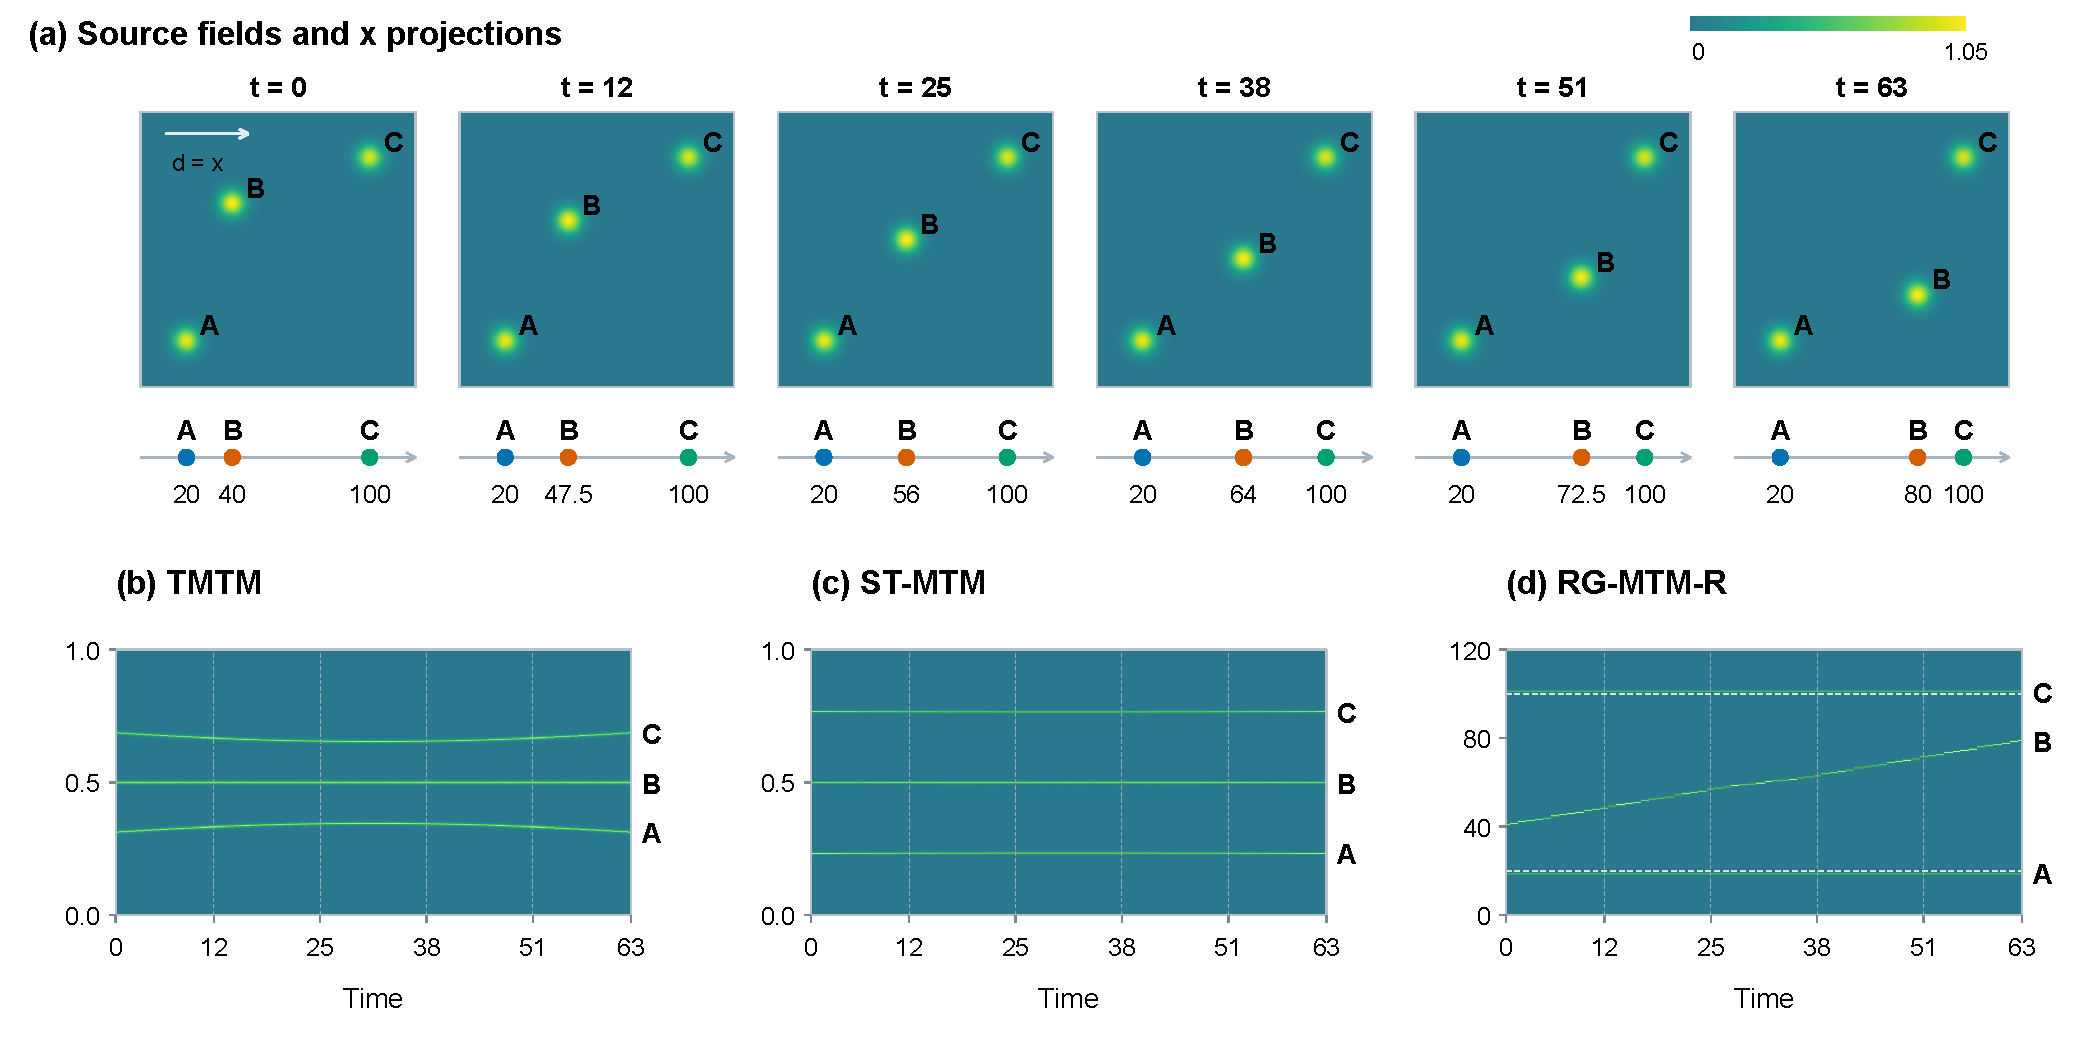
\includegraphics[width=\linewidth]{figures/Supplement_ReferenceControl_Full.pdf}
\caption{Relative distances and absolute reference position. (a) Six source fields and $x$ projections follow moving $B$ between fixed $A,C$; mirror endpoints preserve pairwise distances while changing horizontal position. (b,c) TMTM/ST-MTM use internal map coordinates. (d) RG-MTM-R uses source $x$ units, with dashed fixed references. Source peaks and temporal bands share a linear 0--1.05 scalar scale. Vertical guides mark source-frame times. All three preserve merge levels; position errors and calibration are reported in the main paper's absolute-reference control.}
\label{fig:s_full_bisector_three_methods}
\end{figure}

\begin{figure}[H]
\centering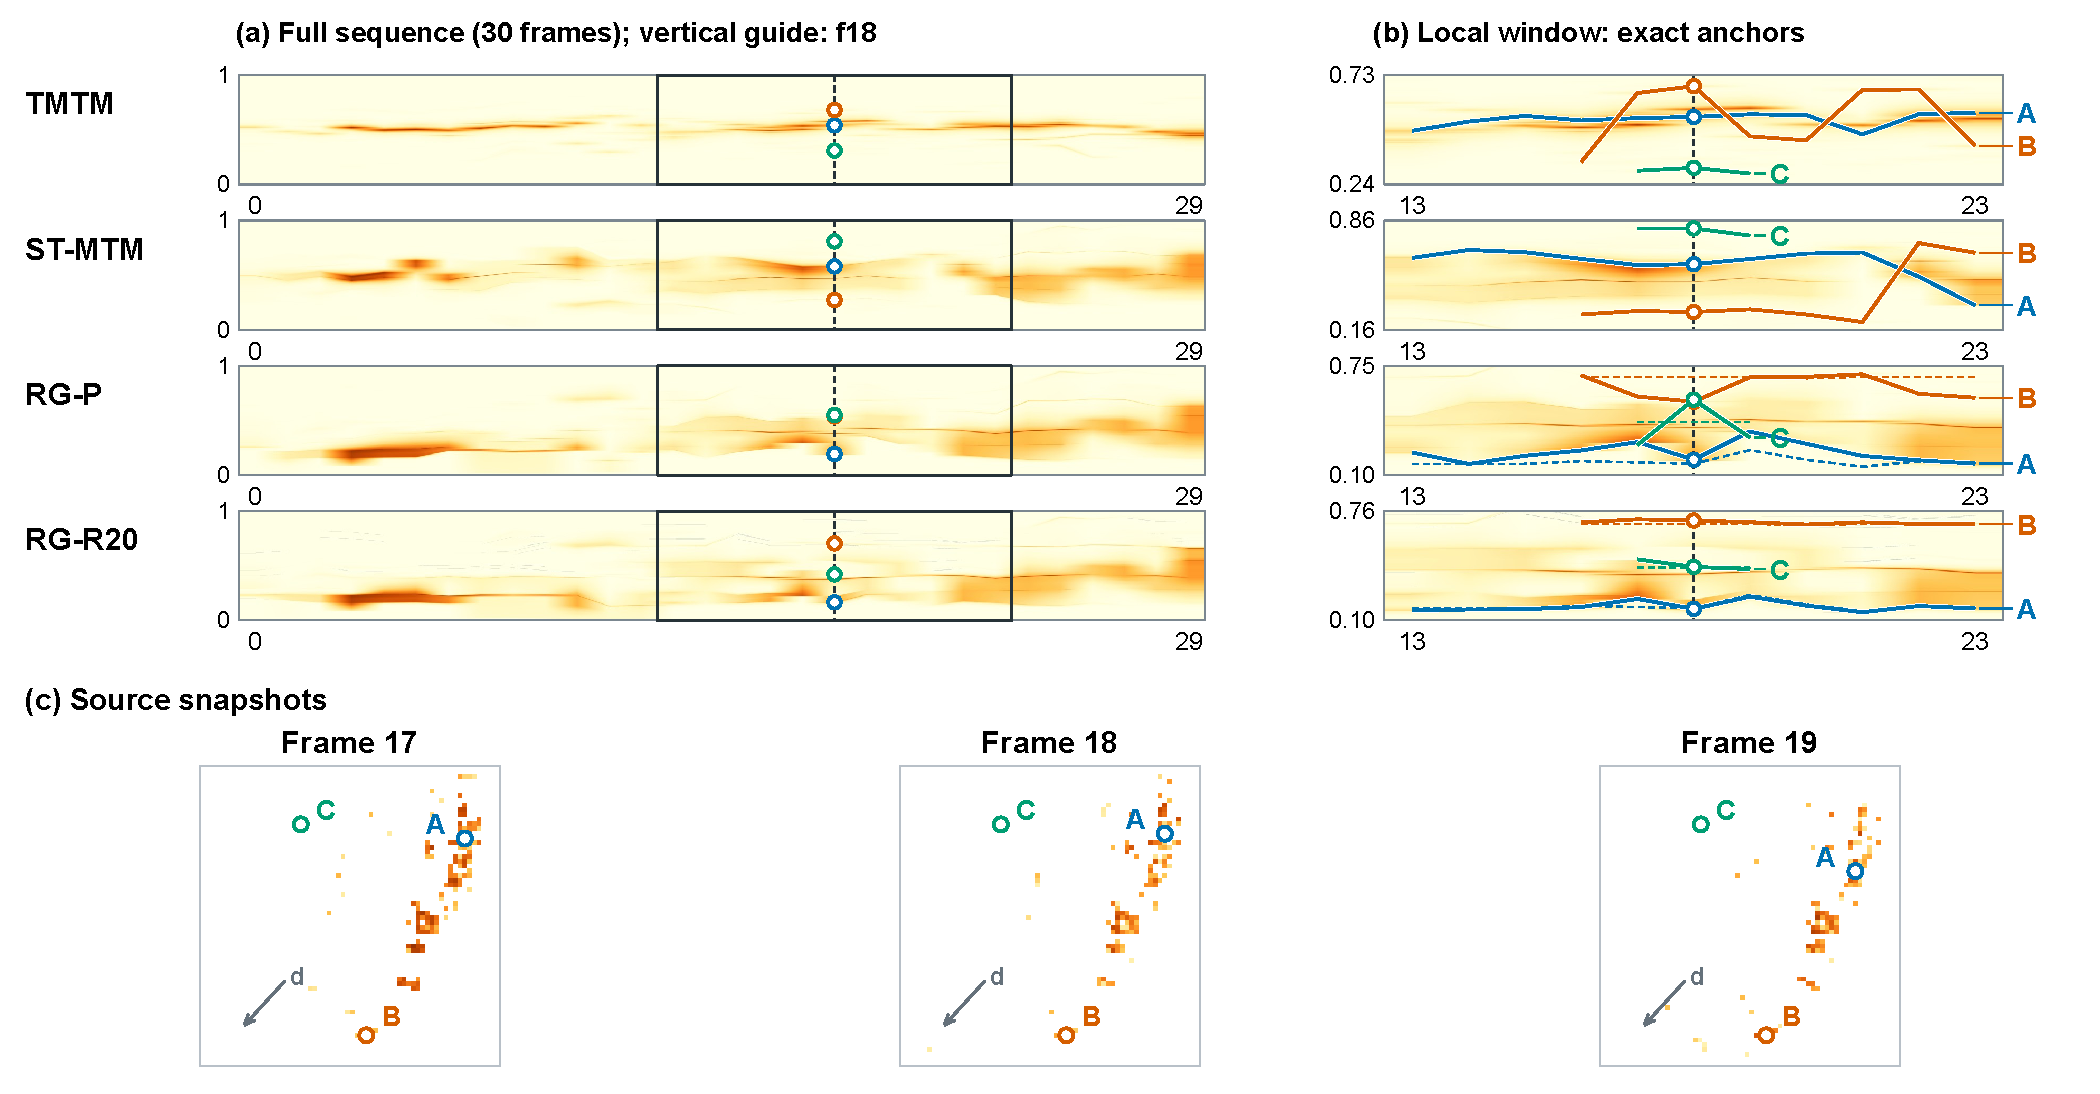
\includegraphics[width=\linewidth]{figures/Supplement_Wildfires_Comparison.pdf}
\caption{Wildfires source events and four layouts. Complete 30-frame maps (left) and frames 13--23 (right) share tracks $A=3$, $B=48$, $C=52$. Circles and solid traces show saved anchors; dashed RG traces show references. Baseline axes are native rank; RG axes use the fixed projection. Local ordinate ranges are labelled. Bottom: two-date FRP sums aggregated onto the $64\times64$ grid and transformed by $\log(1+\mathrm{FRP}/\mathrm{MW})$, before smoothing, at frames 17--19. These are binned records rather than untouched satellite observations or burn perimeters. The overlaid markers locate processed extrema. The main wildfire figure separately displays the supplied 10-km cell polygons with geographic context and the corresponding smoothed analysis fields. At frame 18, P/R maximum displacement is 14.75\%/2.63\% of reference extent, at 15.09\% actual R NMLE. A yellow--orange--brown scale encodes log-FRP with fixed ranges 0--4.21 for processed maps and 0--12.05 for binned snapshots. Grey-blue denotes artificial negative connections. Temporal colour maps use display interpolation only; source snapshots and all original evaluation samples are unchanged.}
\label{fig:s_full_wildfires_events}
\end{figure}

\begin{figure}[H]
\centering\includegraphics[width=\linewidth]{figures/Supplement_OLR_Comparison.pdf}
\caption{OLR: complete 60-frame frozen method maps on one scalar scale. Baseline ordinates are native sample rank, while P/R use the fixed reference; normalization of the displayed axes does not make their meanings identical. The common primary motion record gives P and R20 the same total of 3/56 errors, despite improved reference order. No local temporal crop is selected.}
\label{fig:s_olr_complete}\end{figure}
\begin{figure}[H]
\centering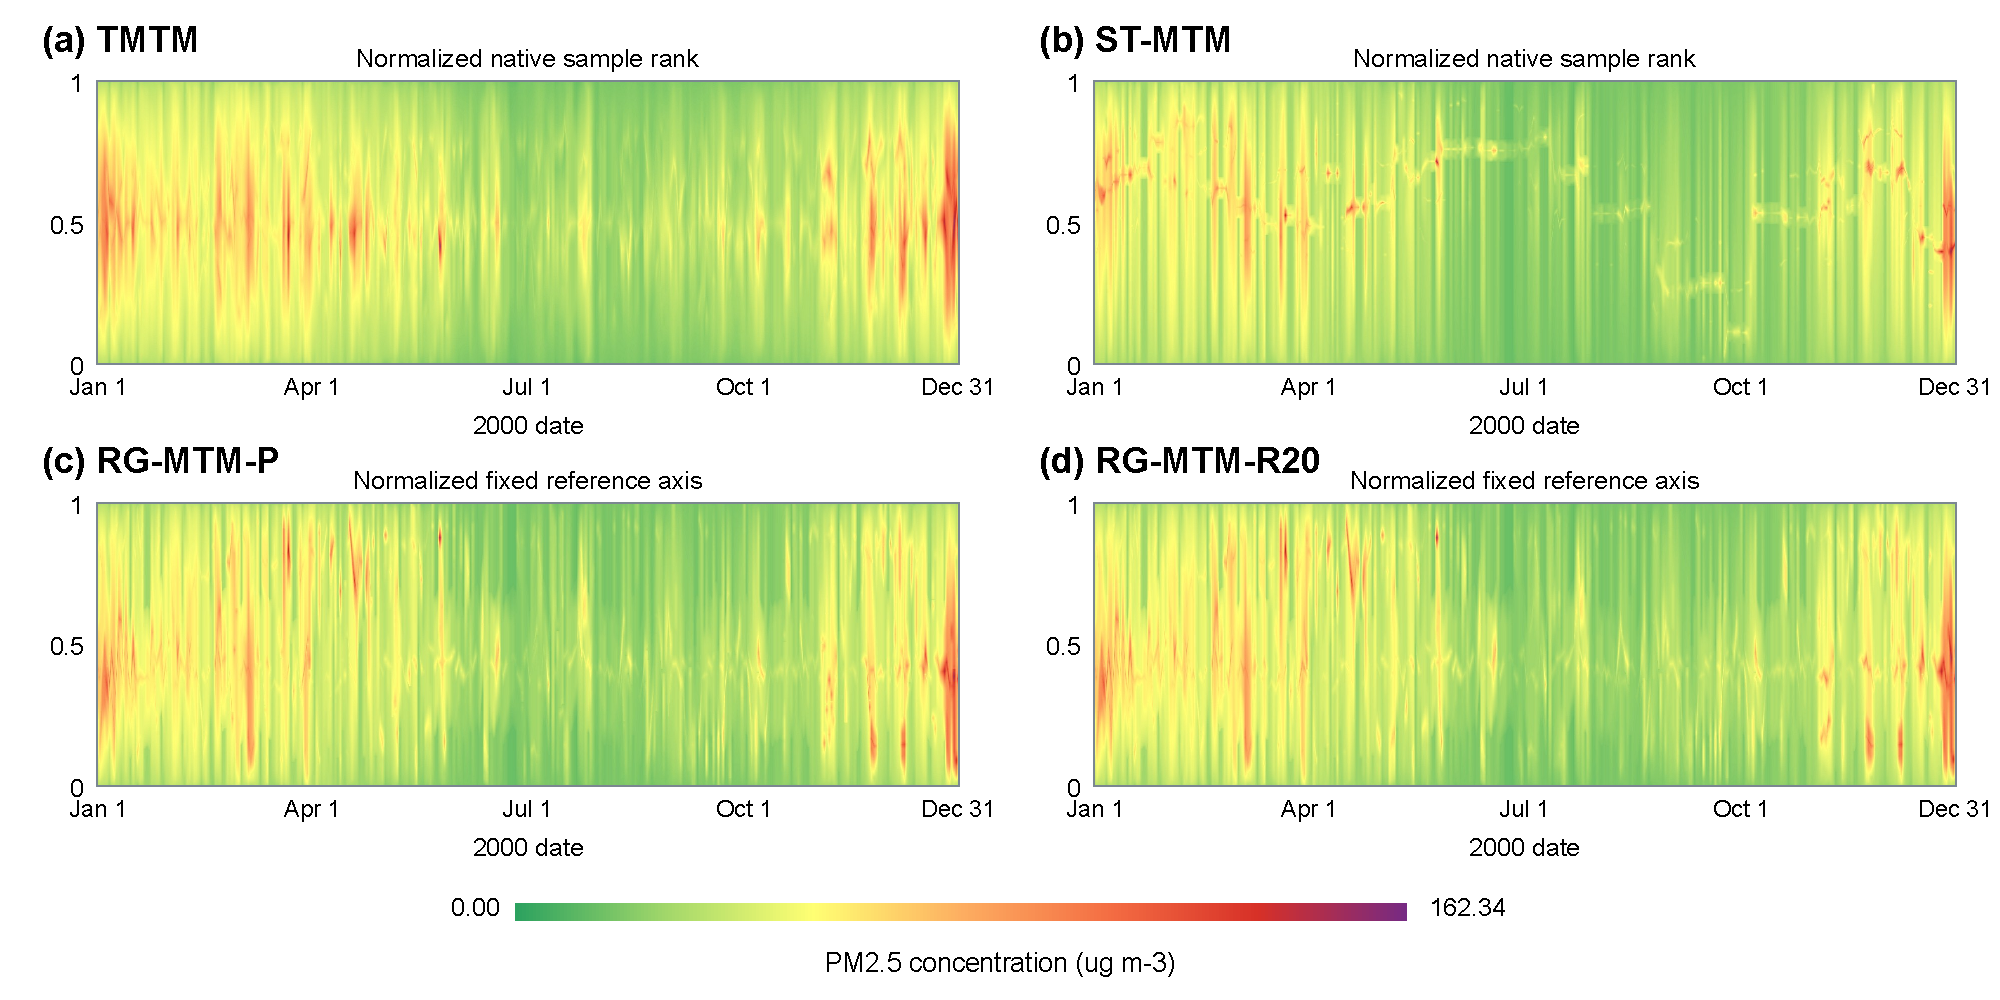
\includegraphics[width=\linewidth]{figures/Supplement_PM25_Comparison.pdf}
\caption{PM2.5: complete 2000 sequence (366 fields) for TMTM, ST-MTM, P and R20. All methods share the same processed inputs. Native baseline rank axes differ from the fixed RG reference axis. The shared pollution palette encodes concentration, not AQI. Conservative interpolation preserves every saved profile; metrics use original arrays. P/R20 motion errors are 42/95 and 47/95 on continuous anchors. The annual result replaces the earlier January display.}
\label{fig:s_pm25_complete}\end{figure}

\begin{figure}[H]
\centering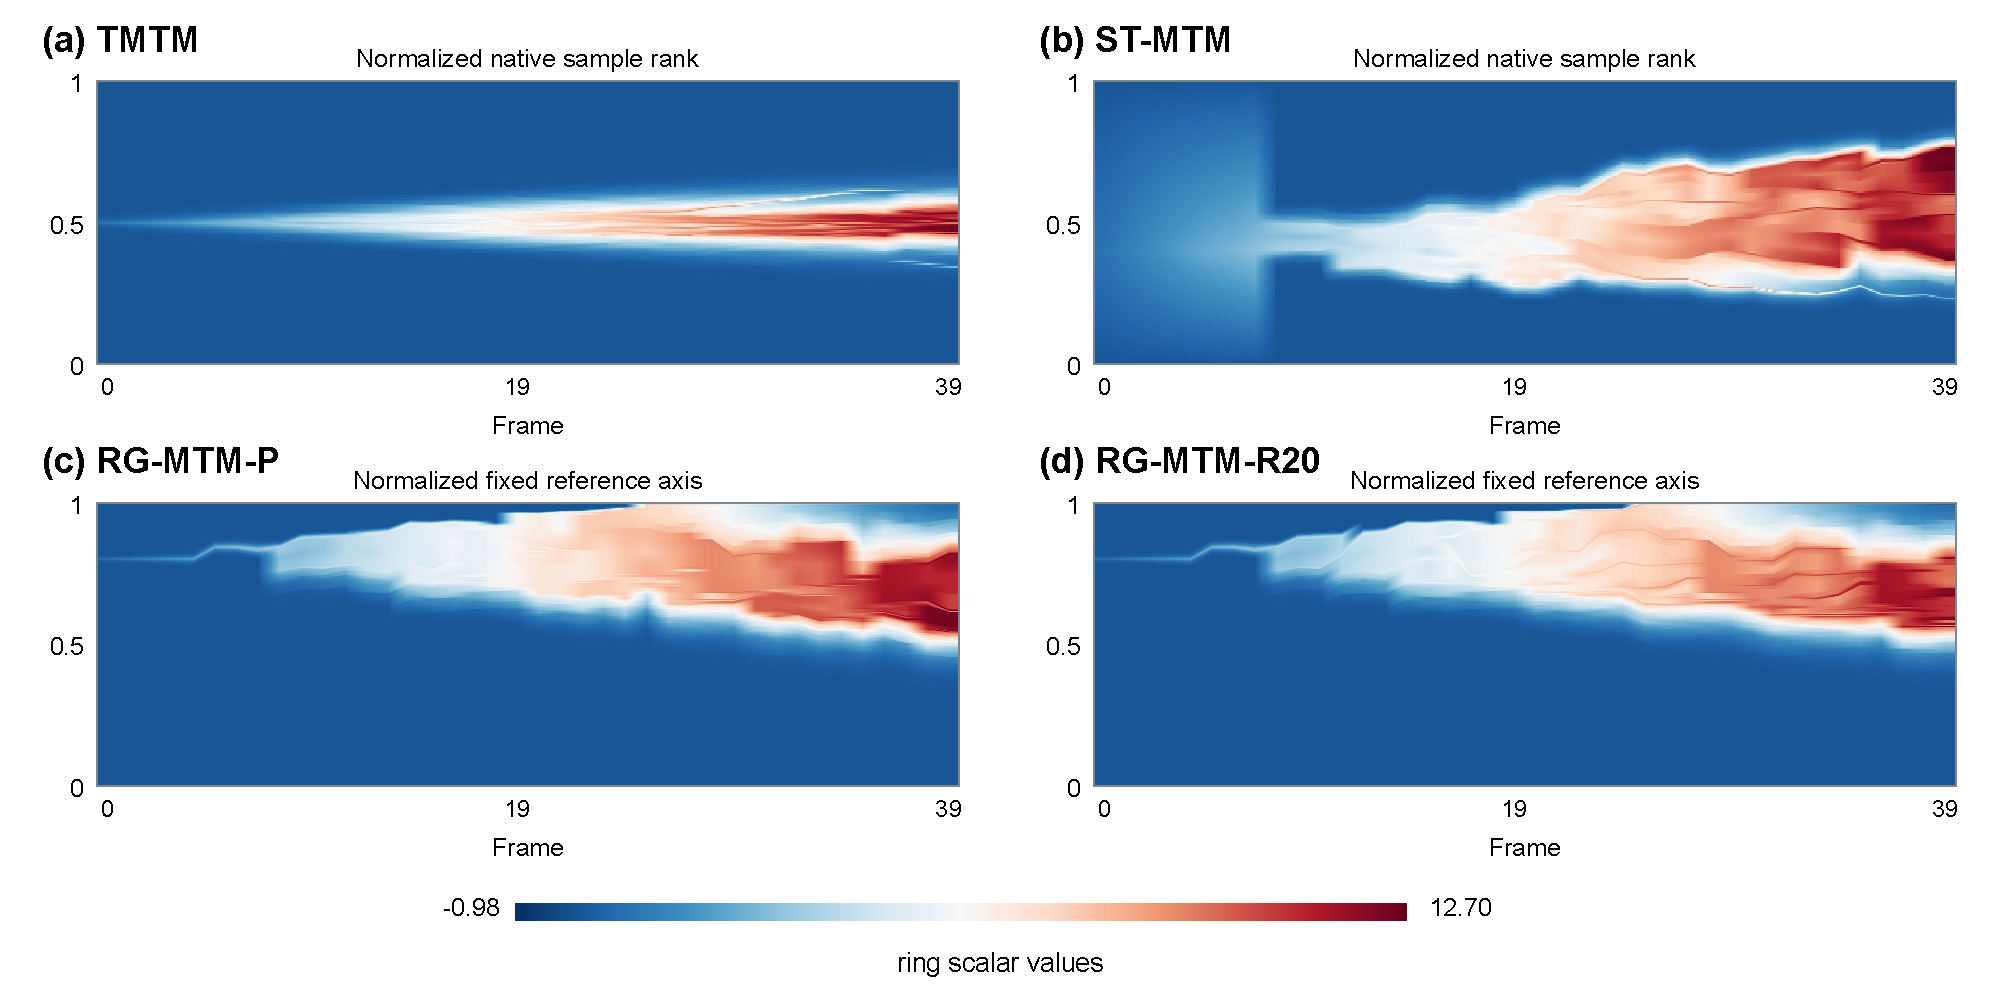
\includegraphics[width=\linewidth]{figures/Supplement_Ring_Comparison.pdf}
\caption{Ring: all 40 saved frames for TMTM, ST-MTM, P, and R20 on a shared scalar scale. Baseline ordinates are normalized native sample rank; P/R use the fixed spatial reference. Their meanings remain distinct. R20 improves the primary spatial-motion proxy from P's 39/124 to 16/124 at 2.73\% mean NMLE. This is the archived author ring generator on a $14\times14$ grid. Source hashes and zero cross-method scalar residuals at 165 saved feature anchors bind the displayed cache to the retained experiment; no layouts were recomputed.}
\label{fig:s_ring_complete}
\end{figure}

\begin{figure}[H]
\centering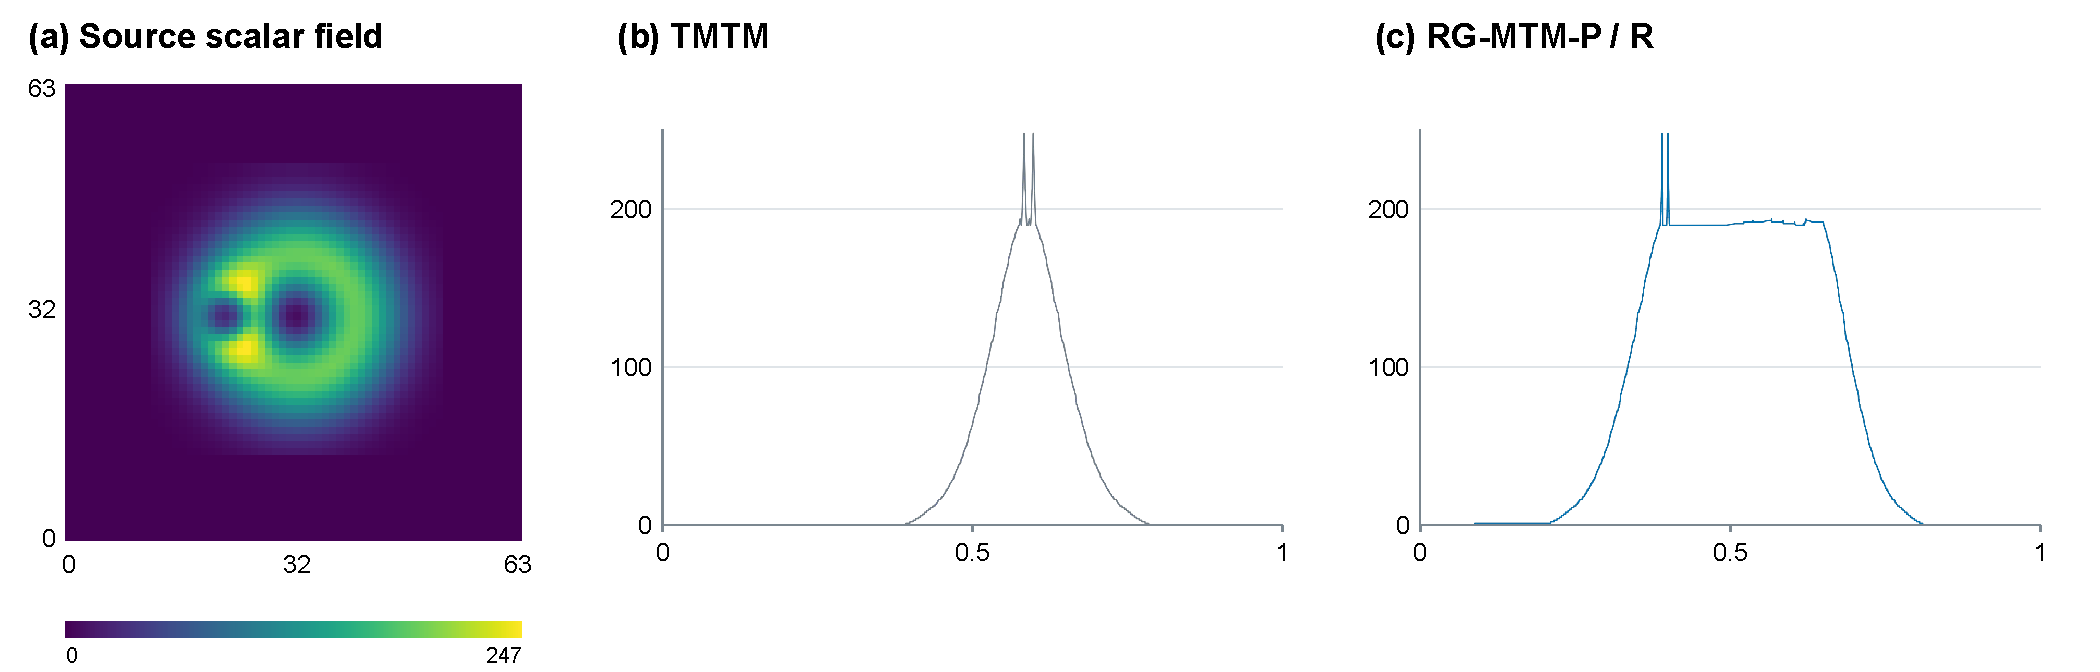
\includegraphics[width=\linewidth]{figures/Supplement_Nucleon_Comparison.pdf}
\caption{Nucleon static comparison. (a) The unchanged author $64\times64$ scalar slice. (b) Complete TMTM profile (4096 samples). (c) Complete P profile (32768 samples); all three R profiles are exactly identical to P. The source and curves use the original scalar units. NROE decreases from 11.90\% to 2.38\%, with zero measured NMLE throughout. This single frame supplies no temporal-motion or three-dimensional result.}
\label{fig:s_full_nucleon}
\end{figure}

\begin{figure}[H]
\centering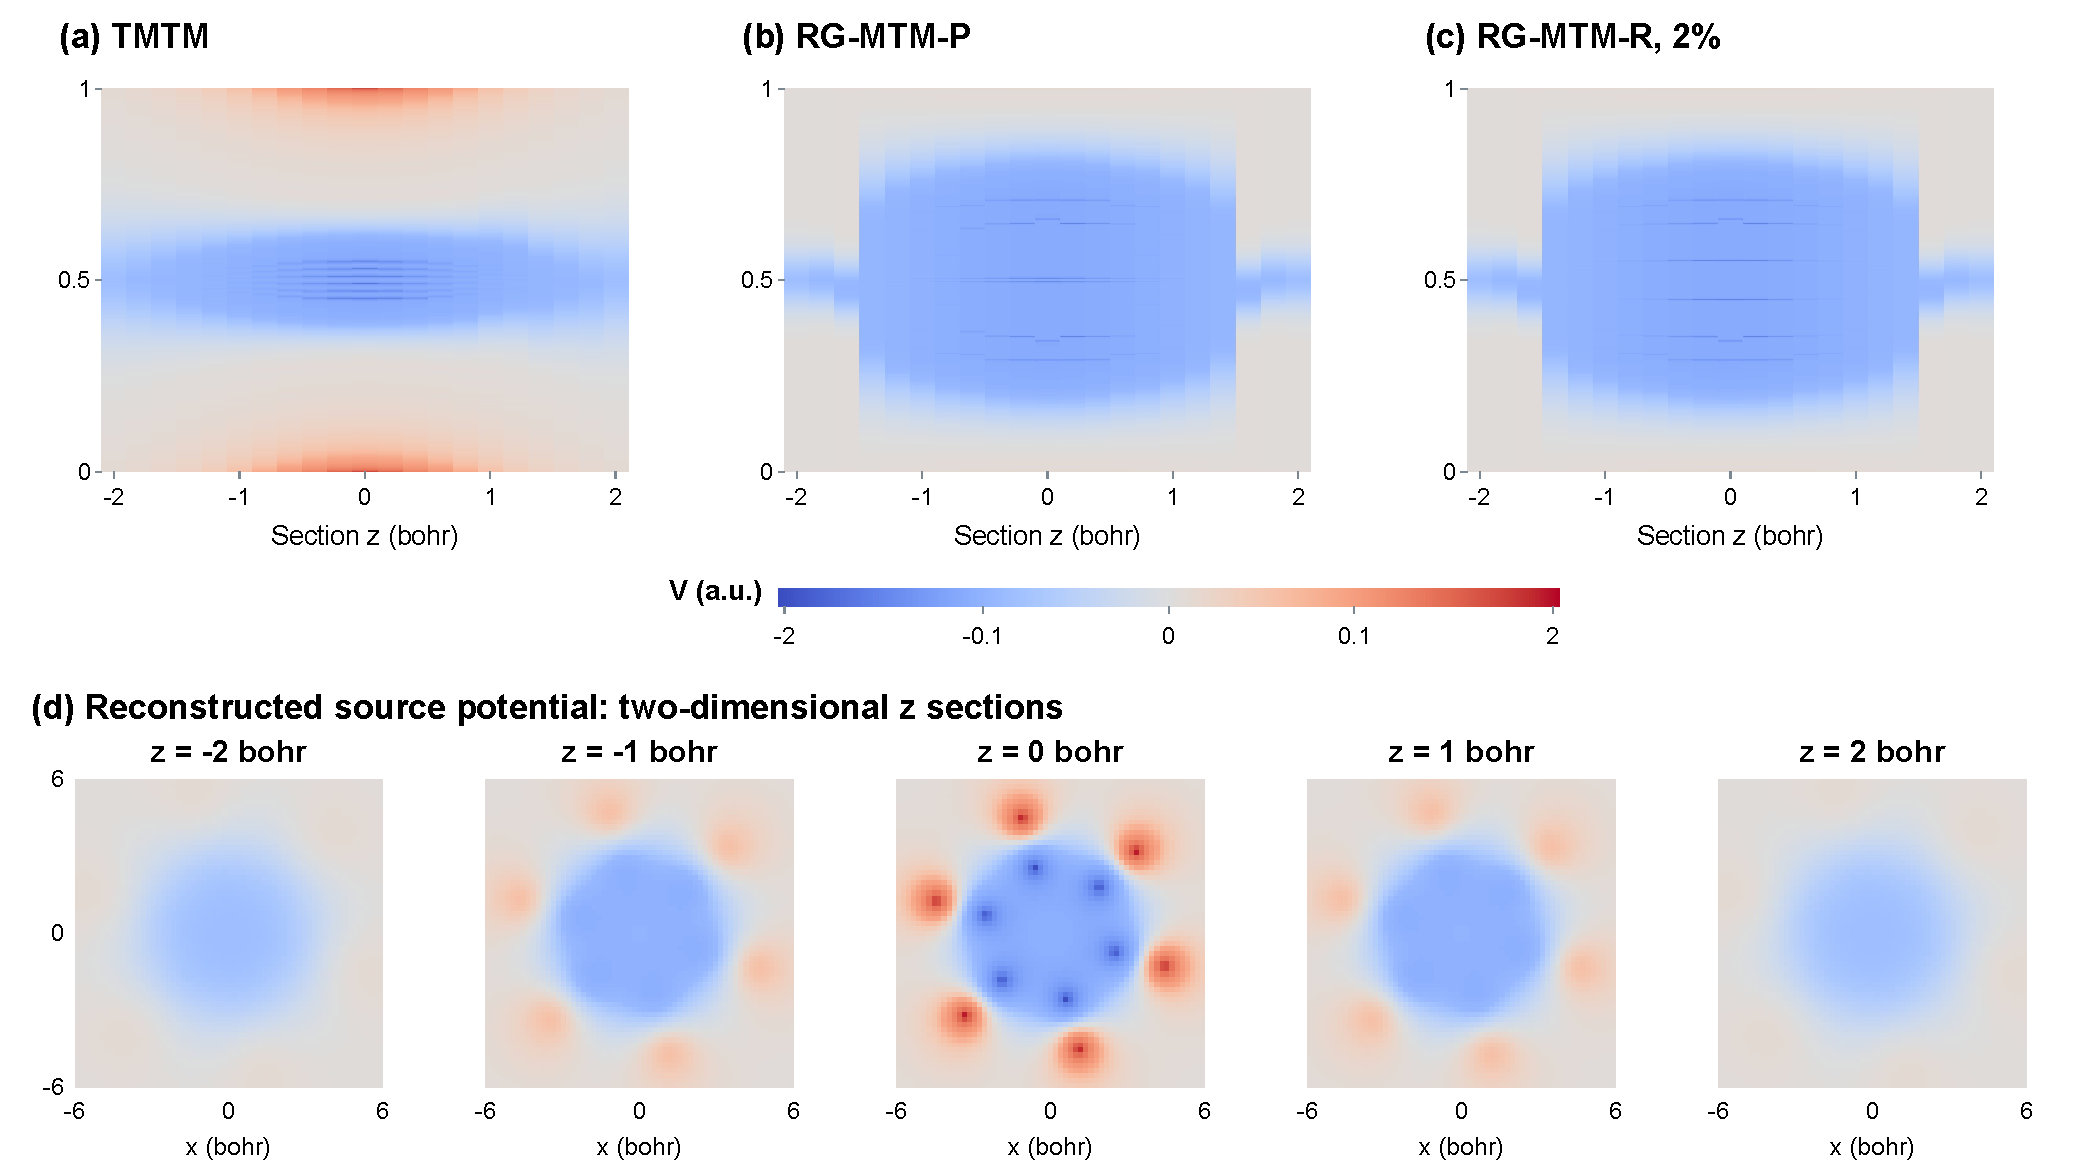
\includegraphics[width=\linewidth]{figures/Supplement_Benzene_Comparison.pdf}
\caption{Benzene reconstructed electrostatic potential. (a)--(c) Maps of all 21 static $z$ sections for TMTM, P, and R2; $z$ is not physical time. TMTM uses its native map coordinate, while RG uses normalized $x$ reference position. (d) Five $61\times61$ source-potential sections on the same symmetric-log colour scale (linear within $\pm0.0784$ a.u.). Values are in Hartree/$e$; source coordinates are in bohr. The field is the declared OPLS-AA point-charge reconstruction, not the original author's potential or electron density. Full-population scores retain four boundary extrema per section; internal-extremum diagnostics are reported separately.}
\label{fig:s_full_benzene}
\end{figure}

\begin{figure}[H]
\centering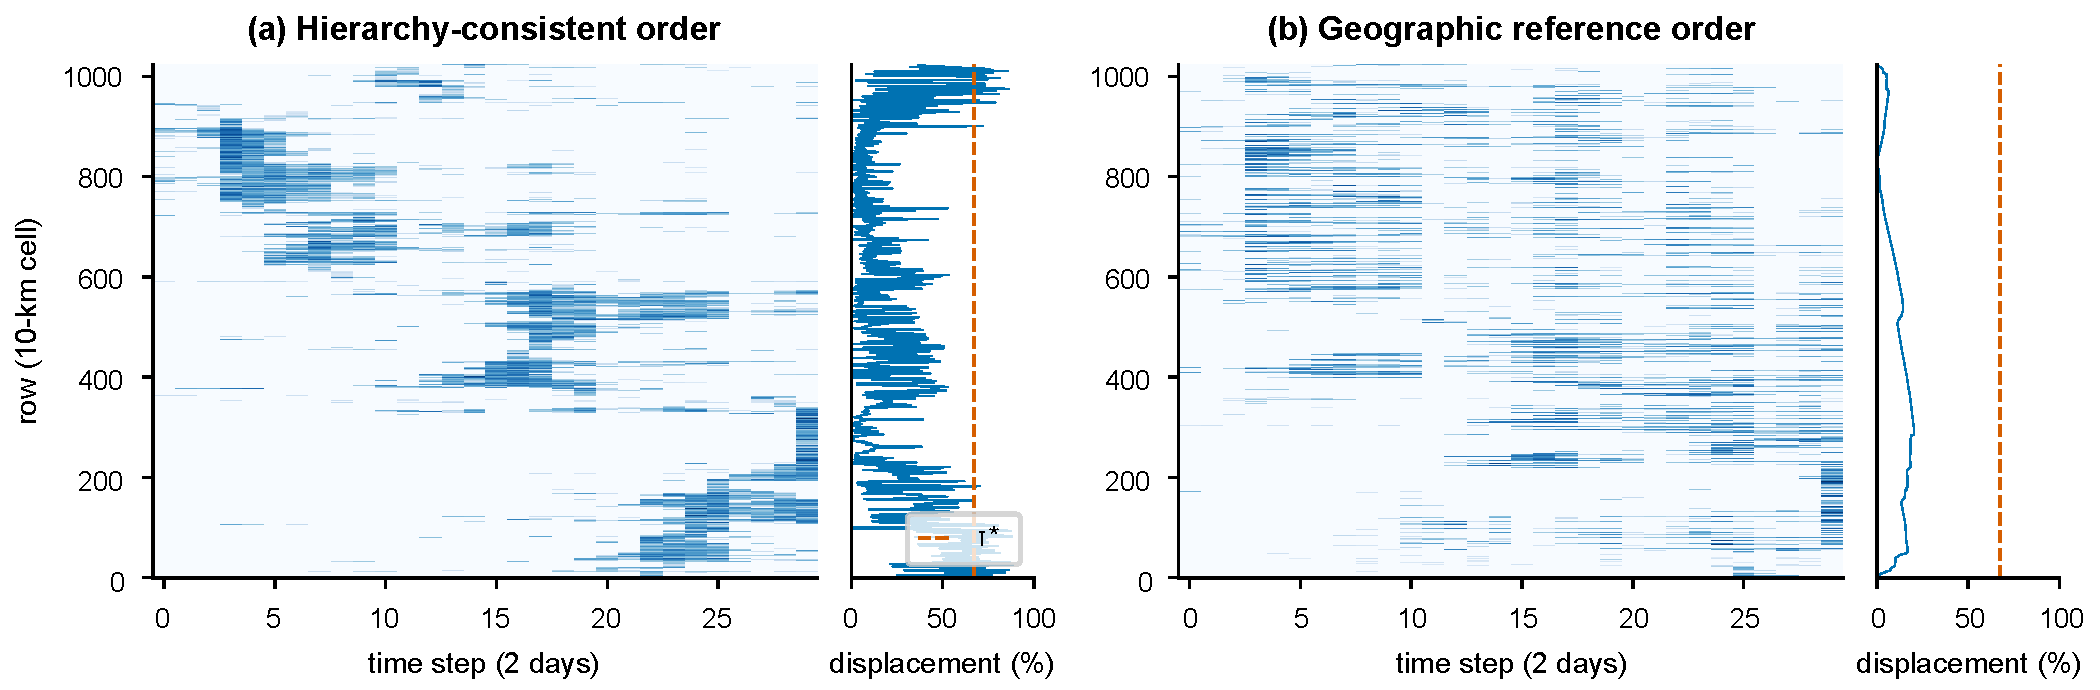
\includegraphics[width=\linewidth]{figures/Supplement_Dendrogram_Transfer.pdf}
\caption{Position certification for a clustering hierarchy of 1024 active wildfire cells. The same 30 two-day $\log(1+\mathrm{FRP})$ observations are arranged in dendrogram-consistent optimal leaf order (a) and in geographic reference order (b). Blue encodes signal magnitude; each cell occupies one row. Side panels show absolute displacement from the cell's principal-axis geographic reference, normalized by 1024 rows. The dashed line marks the hierarchy-constrained optimum $\tau^*\approx67.29\%$ (computed to 0.25 row). Observed maxima are 88.23\% for OLO and 20.55\% for geographic sorting, the free-packing optimum. Their separation distinguishes ordering choice from the additional cost imposed by hierarchy.}
\label{fig:s_dendrogram_transfer}
\end{figure}

The positional certificate extends to clustering hierarchies in dense temporal displays. Figure~\ref{fig:s_dendrogram_transfer} arranges 1024 active 10-km wildfire cells~\cite{Franke:2021:1DP}, each as one row containing 30 two-day $\log(1+\mathrm{FRP})$ observations. Average-linkage clustering of centered, unit-normalized temporal signals defines the dendrogram; optimal leaf ordering (OLO) groups similar signals within its legal orders. Reference positions project cell locations onto the principal geographic axis and span row centers $0.5$--$1023.5$. Both panels contain the same observations and use identical row widths and color mapping.

OLO groups temporally similar activity into visible bands but displaces some cells by 88.23\% of display height. Positional diagnosis over all dendrogram-consistent orders gives $\tau^*/n\approx67.29\%$, where $n=1024$. The approximately 20.94-percentage-point gap separates the chosen ordering's displacement from the minimum imposed by this hierarchy: changing the leaf-ordering algorithm can improve position, while subtree contiguity still prevents accurate geographic placement.

Geographic sorting removes the contiguity constraints and attains $\tau_{\free}/n=20.55\%$. Equal-width rows fill the canvas, so nonuniform geographic references still incur packing cost. The hierarchy contributes the additional $H/n=(\tau^*-\tau_{\free})/n\approx46.73\%$ of display height, or 46.73 percentage points beyond packing. Together with the mirror control, this distinguishes two sources of positional ambiguity: distances alone do not fix absolute references, and a fixed hierarchy can obstruct those references even under optimal positional ordering. The row experiment transfers positional diagnosis to a 1024-leaf clustering tree; the merge-tree experiments quantify scalar correction and relaxation costs. Supplement S3 gives the numerical precision and retained records.


\subsection{Three-dimensional inputs}
\begin{figure}[H]
\centering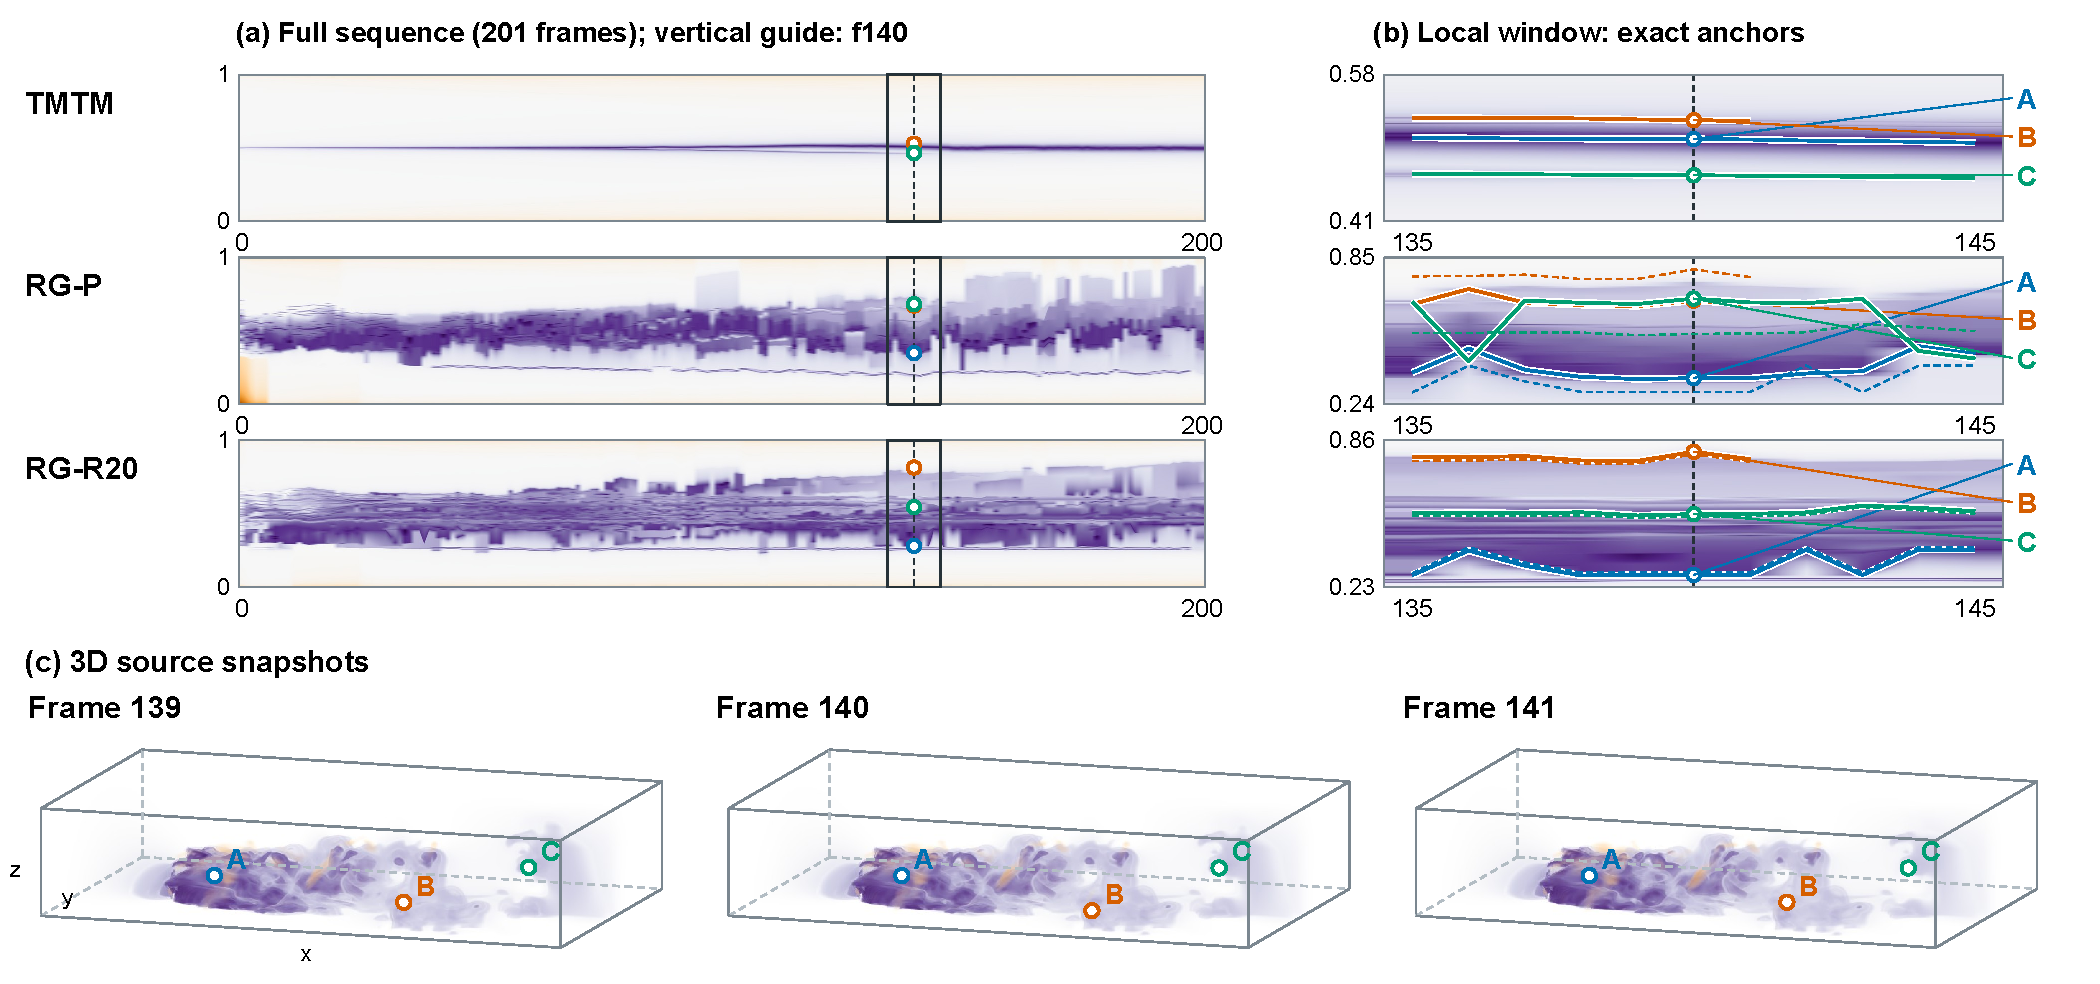
\includegraphics[width=\linewidth]{figures/Supplement_Tangaroa_Comparison.pdf}
\caption{Tangaroa feature correspondence: all 201 original-grid frames at fixed 10\% persistence. Complete TMTM/P/R20 maps (left) link to frames 135--145 (right); tracks $A=432$, $B=462$, $C=388$ use exact saved anchors and dashed RG references. Baseline and RG ordinates retain their distinct meanings. Bottom: cached full-volume views at frames 139--141, with domain boxes and true extrema projected through one shared oblique orthographic camera. Preview layers use 4096 rows; errors use complete 131072-row profiles. At frame 140, P/R maximum displacement is 14.76\%/1.02\%, and R incurs 13.75\% NMLE. Maps and volumes use the retained purple--white--orange speed transfer function over $[0,2]$. Temporal transitions interpolate saved profiles for display only; anchors, input volumes, and evaluation samples are unchanged.}
\label{fig:s_full_volume3d}
\end{figure}

\begin{figure}[H]
\centering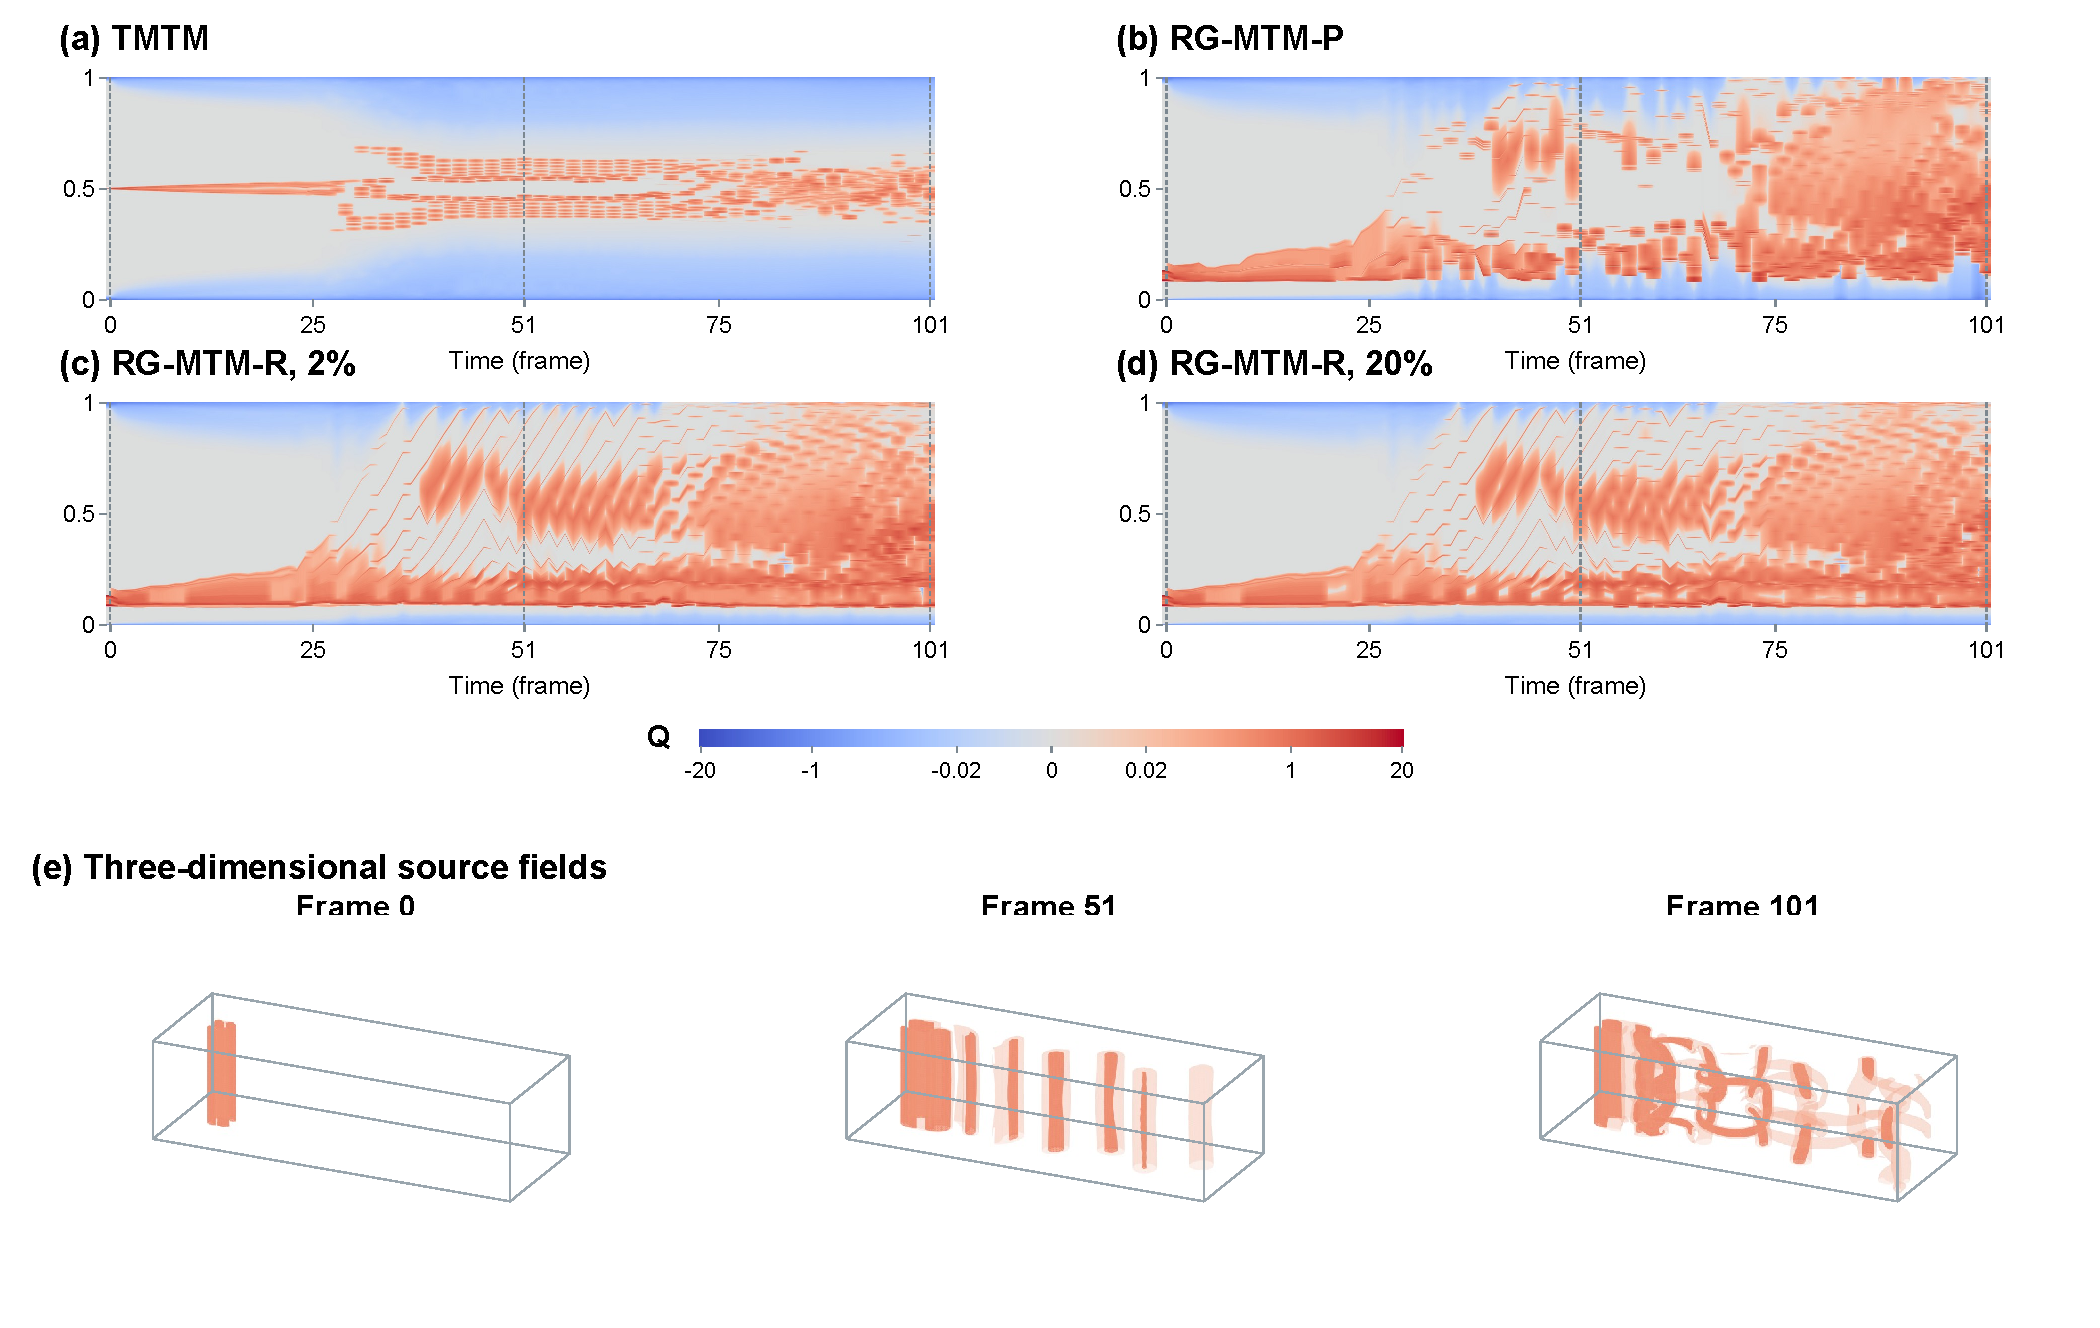
\includegraphics[width=\linewidth]{figures/Supplement_Cylinder_Comparison.pdf}
\caption{Cylinder: 102 original-grid three-dimensional $Q$ fields. (a)--(d) Saved scalar maps for TMTM, P, R2, and R20; TMTM uses a native ordinate, while RG uses normalized physical $x$ reference position. Dashed guides locate frames 0, 51, and 101. The common symmetric-log colour scale is linear within $\pm0.02$; the revised raster integrates complete stored profiles vertically rather than selecting 2048 rows. Temporal colour transitions are display interpolation; metrics use the original arrays. (e) Three-dimensional source isosurfaces at $Q=0.1$ (translucent) and $0.5$ (solid), with identical physical aspect, orthographic camera, and domain frame. They show the source $Q$ before persistence simplification; maps use the shared simplified inputs and their stated scalar fillings.}
\label{fig:s_full_cylinder}
\end{figure}
